\subsection{Two Failure Mechanisms Along the Load Axis}\label{sec:num-loadaxis}
This set of experiments covers 32 configurations and about 1.69 million failure samples. We split failures into two
layers according to the actual core: a macroscopic layer (the core contains more than $0.1d$ edges) and a
repeated-edge layer (the core contains a pair of identical edges); the classification criterion is stated in
Section~\ref{sec:exp-design}.

The repeated-edge layer is further grouped by the sign product $\sigma$; its conditional mean equals the
unconditional mean plus $\pm2/s_M$. The largest $|z|$ among the 54 test units is $3.13$. On the macroscopic layer,
the test of the rejection rate of the corrected selection threshold is not rejected in any of the 96 test units; for
$M\ge4096$, rej$/u$ lies between $0.83$ and $1.25$.
The difference between the macroscopic-layer weight computed from the analytic formula and the measured value is at
most $0.032$ for $M\ge4096$, and at most $0.009$ for $M=16384$ and $65536$. These results support the mechanistic
picture described by Proposition~\ref{prop:lowload} and Proposition~\ref{prop:mixture}.

Figure~\ref{fig:twomech} shows the layering results for $k=3$ with all-equal sign. As $z_{\rm sh}$ decreases, the
weight of the macroscopic layer passes from 1 to 0, and the transition location deepens as $M$ grows; the theoretical
curve $\Phi(z_{\rm sh})/(\Phi(z_{\rm sh})+p_{\rm dup})$ contains no adjustable parameters. The
conditional mean of all failures falls to $2/s_M$ of the repeated-edge layer on the low-load side and returns to the
mean given by the macroscopic-layer selection law on the window side.
The ratio of the measured shift of the repeated-edge layer to $2\sigma/s_M$ lies between $0.90$ and $1.05$ for every
$M$ and both values of $\sigma$.
In the region where the macroscopic layer dominates, the conditional mean exceeds the theoretical value by
15\%--60\% at $M=1024$, and drops to 3\%--8\% for $M\ge16384$; this has the same origin as the positive residual of
the macroscopic layer in Appendix~\ref{sec:convergence}.

The conditional probability of the sign product $\Pr(\sigma=+1\mid P_2)=(1+\gamma)/2$ is an exact equality in finite
samples. Under the prespecified criterion, it is rejected on one test unit ($z=-4.45$); rerunning the same
configuration with a new seed gives $z=+1.89$, and the deviation does not recur. The same experiment also reproduces
the failure that occurs when only the corrected selection threshold is used: in the low-load region with $k=3$, the
noncoverage under small-core failure can reach 99 times the nominal value. The two implementation rules of
Section~\ref{sec:rules} are designed precisely for this.
\begin{figure}[!htbp]
\centering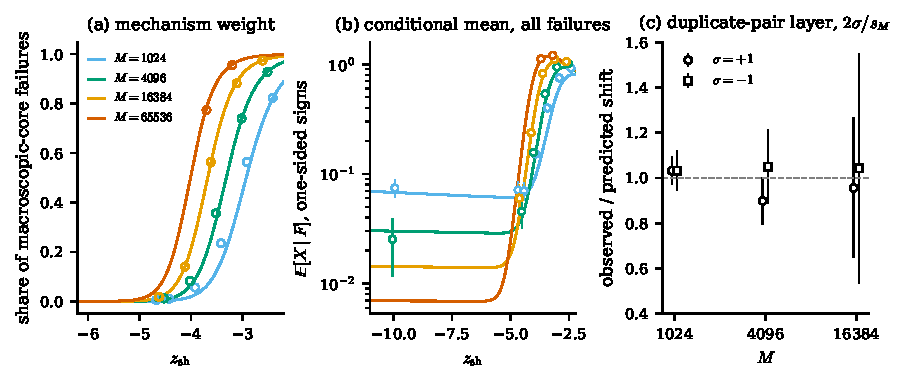
\includegraphics[width=\linewidth]{figures/fig-two-mechanism.pdf}
\caption{$k=3$ low-load two-mechanism layering. (a) Fraction of macroscopic-core failures; (b) conditional
mean of all failures (all-equal sign); (c) ratio of the measured shift of the repeated-edge layer to
$2\sigma/s_M$. All curves are analytic predictions.}
\label{fig:twomech}
\end{figure}
